% C7. Validación espacial
\begin{frame}{Cómo validamos: el modelo se evalúa en zonas de Bogotá que no vio}
  \centering
  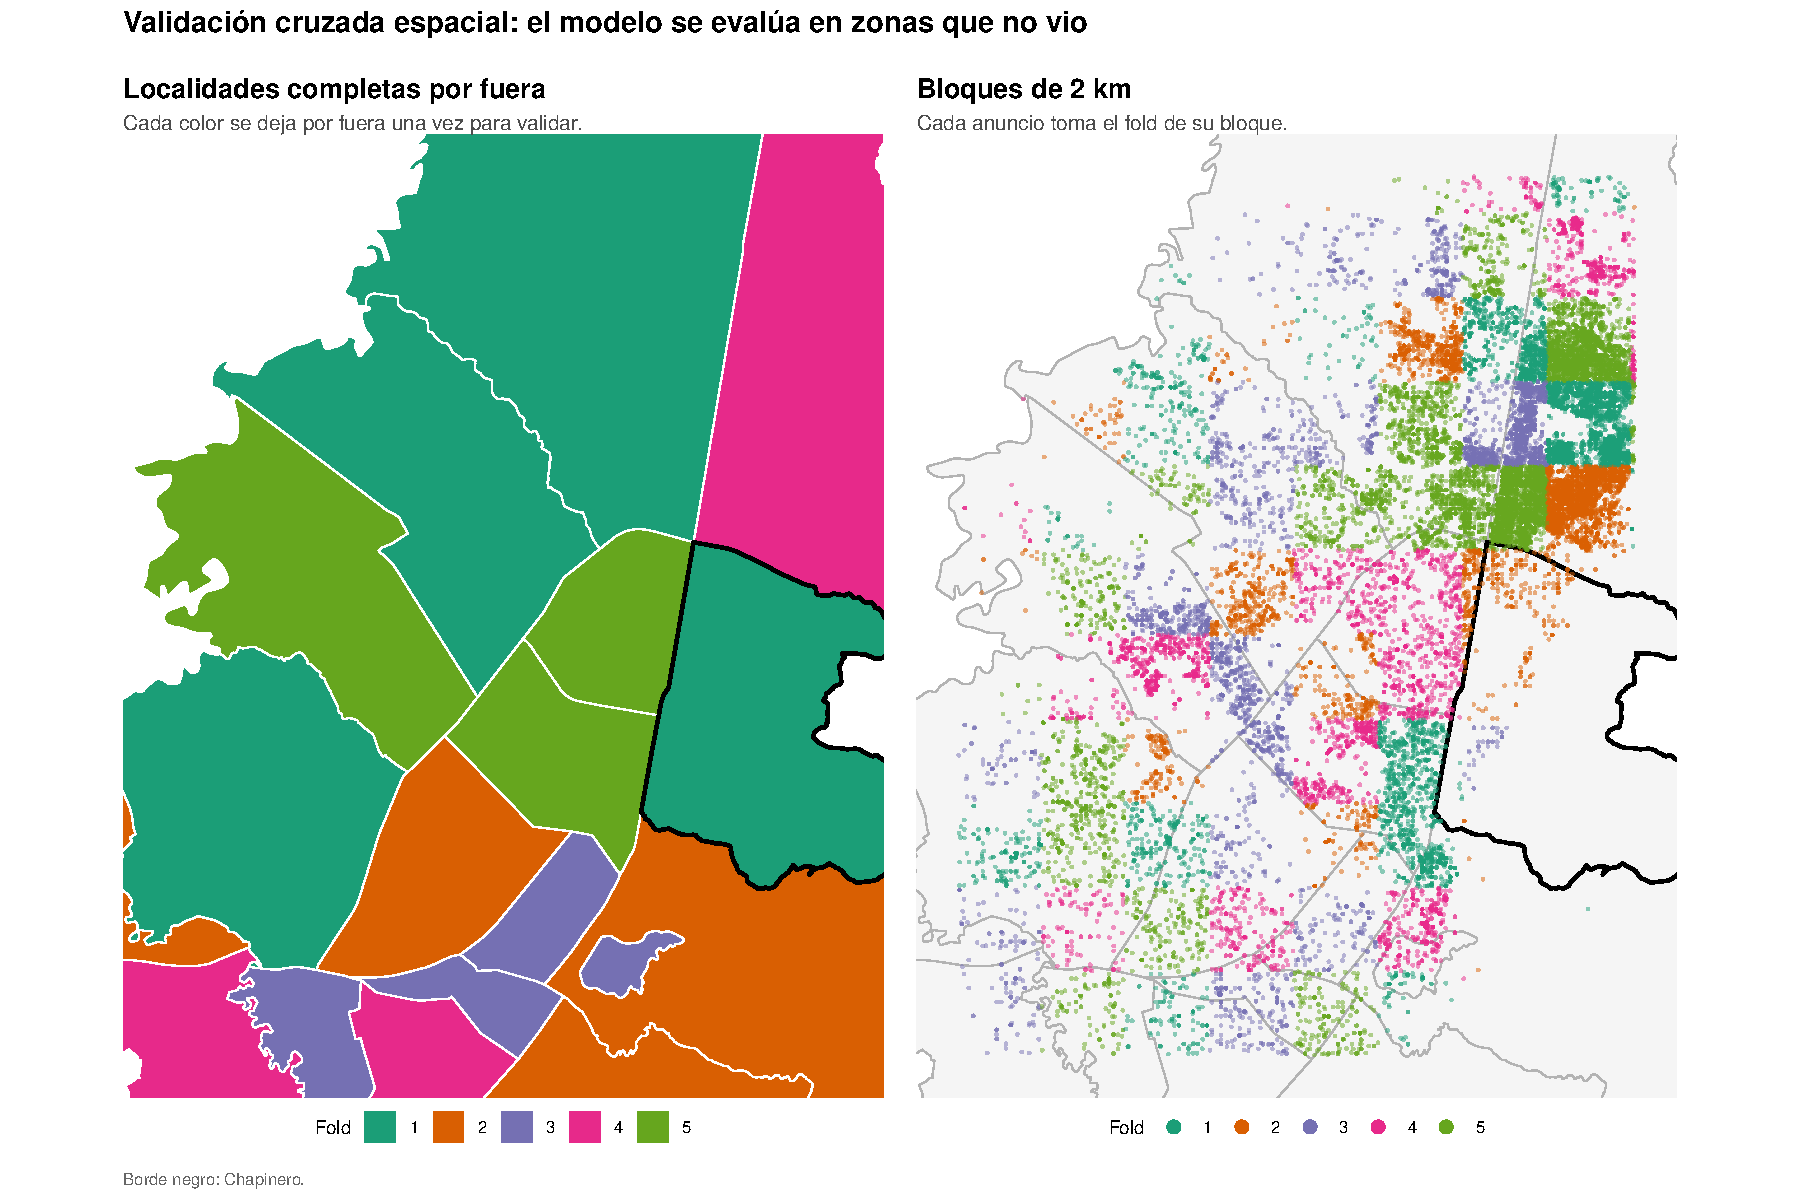
\includegraphics[height=0.86\textheight]{mapa_06_folds_espaciales.pdf}
  \note{En la validación aleatoria, un anuncio de validación casi siempre tiene vecinos en entrenamiento que comparten su precio, y el error se ve más bajo de lo que es. Con localidades completas por fuera, el modelo tiene que predecir una zona que no vio, como pasa con Chapinero. También probamos bloques de 2 km y bloques con un buffer de 300 metros.}
\end{frame}
